\documentclass[12pt]{article}

\usepackage{float}
\usepackage{dsfont}
\usepackage{amsmath}
\usepackage{graphicx}

\usepackage[font=footnotesize,labelfont=bf]{caption}

\usepackage{bm}
\newcommand{\m}[1]{\mathbf{\bm{#1}}}
\newcommand{\R}{I\hspace{-4.4pt}R}

\begin{document}

\noindent AMS 263

\noindent Mickey Warner
\bigskip

\begin{center}
\begin{large}
California precipitation extremes during 1950--1999
\end{large}
\end{center}

\section*{Introduction}

\section*{Methods}

\section*{Results}

\section*{Conclusion}


\noindent The midterm considered the model $\mathcal{M}_0=\{1,1,v,vW_t\}$. This model failed to capture any linear trend or seasonal components in the forecast function. We now consider $\mathcal{M}_1=\{\m{F}, \m{G}, v, v\m{W}_t\}$, where
\begin{eqnarray*}
\m{F} &=& (\m{E}_2^\top, \m{E}_2^\top, \m{E}_2^\top, \m{E}_2^\top, \m{E}_2^\top, \m{E}_2^\top, 1)^\top \\
\m{G} &=& \mathrm{blockdiag}\left(\left(\begin{array}{cc} 1 & 1 \\ 0 & 1 \end{array} \right), \m{G}_1, \m{G}_2, \m{G}_3, \m{G}_4, \m{G}_5, -1 \right)
\end{eqnarray*}
\noindent with
\begin{eqnarray*}
\m{E}_2 &=& (1, 0)^\top \\
\m{G}_j &=& \left(\begin{array}{cc} cos(2\pi j/p) & sin(2\pi j/p) \\ -sin(2\pi j/p) & cos(2\pi j/p) \end{array}\right)
\end{eqnarray*}
\noindent where $p=12$ is the fundamental period. The first two elements of $\m{F}$ correspond to the second-order polynomial trend (which results in the first-order trend in the forecast), and the remaining 11 elements are for the seasonal components. The $\m{G}$ matrix is similar. We also let $\m{W}_t$ be specified using a discount factor $\delta$, $\m{W}_t=(1-\delta)/\delta\m{G}\m{C}_{t-1}\m{G}^\top$. $\m{C}_{t-1}$ is the prior scaling matrix for $\m{\theta}_{t-1}|\mathcal{D}_{t-1}$.
\bigskip

\noindent We use the following priors
\begin{eqnarray*}
\m{\theta}_0|\mathcal{D}_0 &\sim& T_{n_0}(\m{m}_0, \m{C}_0) \\
v|\mathcal{D}_0 &\sim& IG(n_0/2,d_0/2)
\end{eqnarray*}
\noindent with $\m{m}_0=(60, \m{0}_{12}^\top)^\top$, $\m{C}_0=200\m{I}_{13}$, $n_0=1$, and $d_0=100$.These are comparable to the priors I used for $\mathcal{M}_0$ and should be fairly noninformative. Posteriors are obtainined using FFBS.

\subsection*{Analysis}

\noindent The discount factor $\delta$ is selected by maximizing the observed predictive density
\[ p_1(\m{y}|\mathcal{D}_0) = \prod_{t=1}^T p_1(y_t|\mathcal{D}_{t-1}) \]
\noindent The subscript $1$ denotes we are working under $\mathcal{M}_1$. We evaluate $\log p_1(\m{y}|\mathcal{D}_0)$ on the grid $\delta=\{0.800, 0.801,\ldots,1.000\}$. The plot of $\delta$ vs. $\log p_1(\m{y}|\mathcal{D}_0)$ is given in Figure 1. The vertical line marks where the maximum occurs, at $\hat{\delta}_1=0.945$, our selected discount factor. Note, $\log p_1(\m{y}|\mathcal{D}_0)=-478.9$, at $\hat{\delta}_1$.
\bigskip

\begin{figure}[H]
\begin{center}
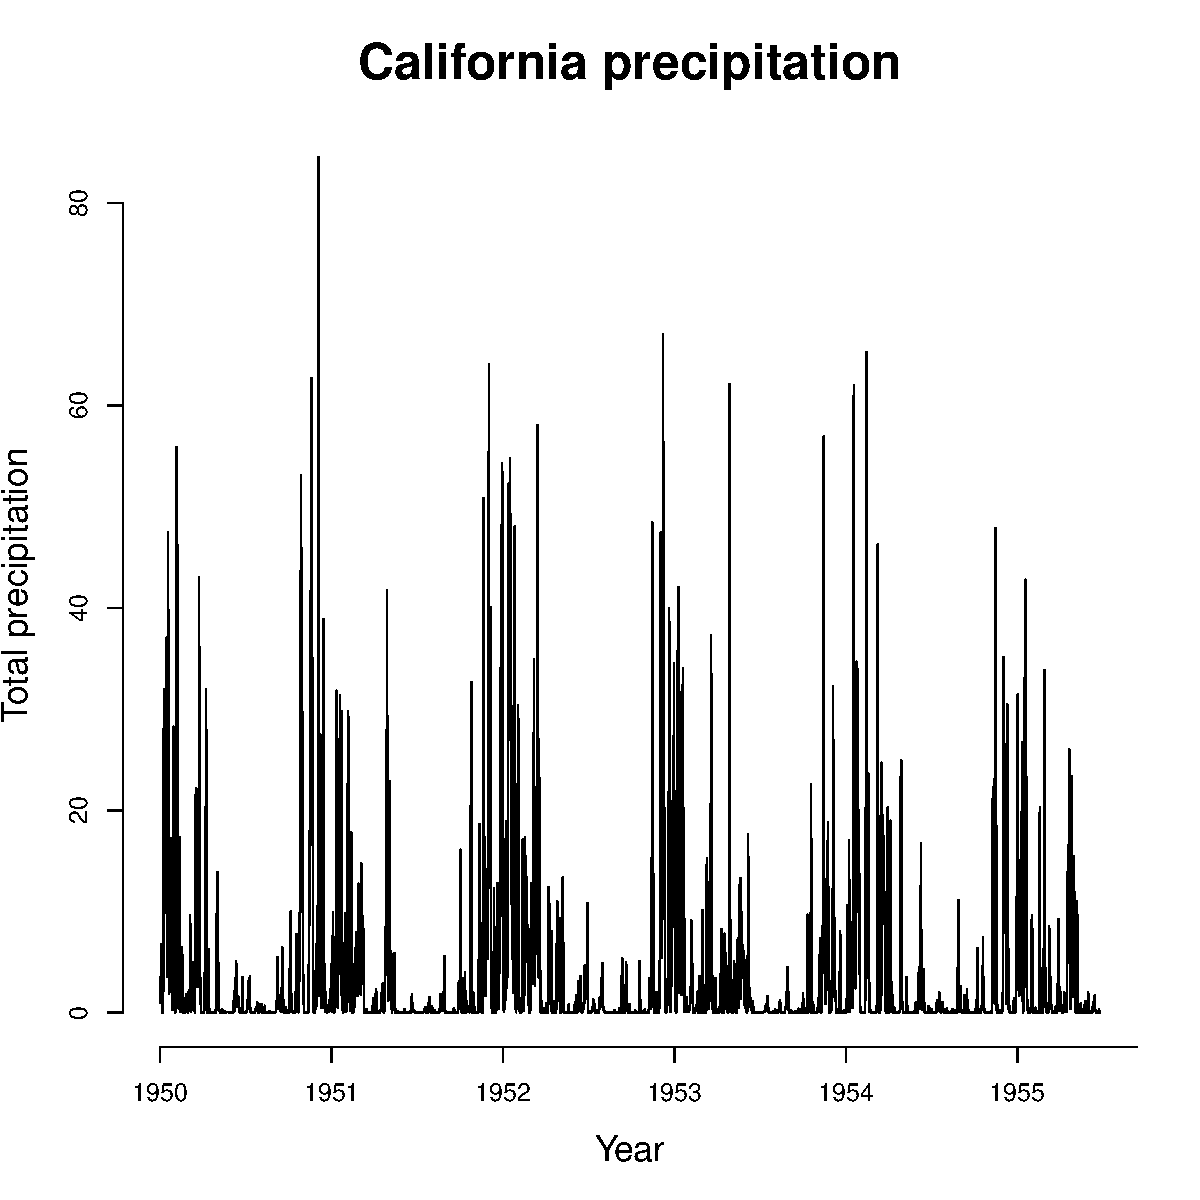
\includegraphics[scale=0.34]{../figs/data.pdf}
\end{center}
\caption{The log observered predictive density evaluated across several $\delta\in[0,1]$. The dashed line indicates where the maximum occurs, at $\hat{\delta}_1=0.945$.}
\end{figure}

\noindent The one-step ahead distribution $y_t|\mathcal{D}_{t-1}$ is summarized in Figure 2. A five-year forecast is shown in Figure 3. The marginal filtering distributions for the trend and the seasonal components (i.e. $\theta_{t,1}$ and $\theta_{t,3}, \theta_{t,5}, \theta_{t,7}, \theta_{t,9}, \theta_{t,11}$ conditioned on $\mathcal{D}_t$) are given in Figure 4. The smoothing distributions (i.e. conditioned on $\mathcal{D}_T$) are in given in Figure 5.
\bigskip

\begin{figure}[H]
\begin{center}
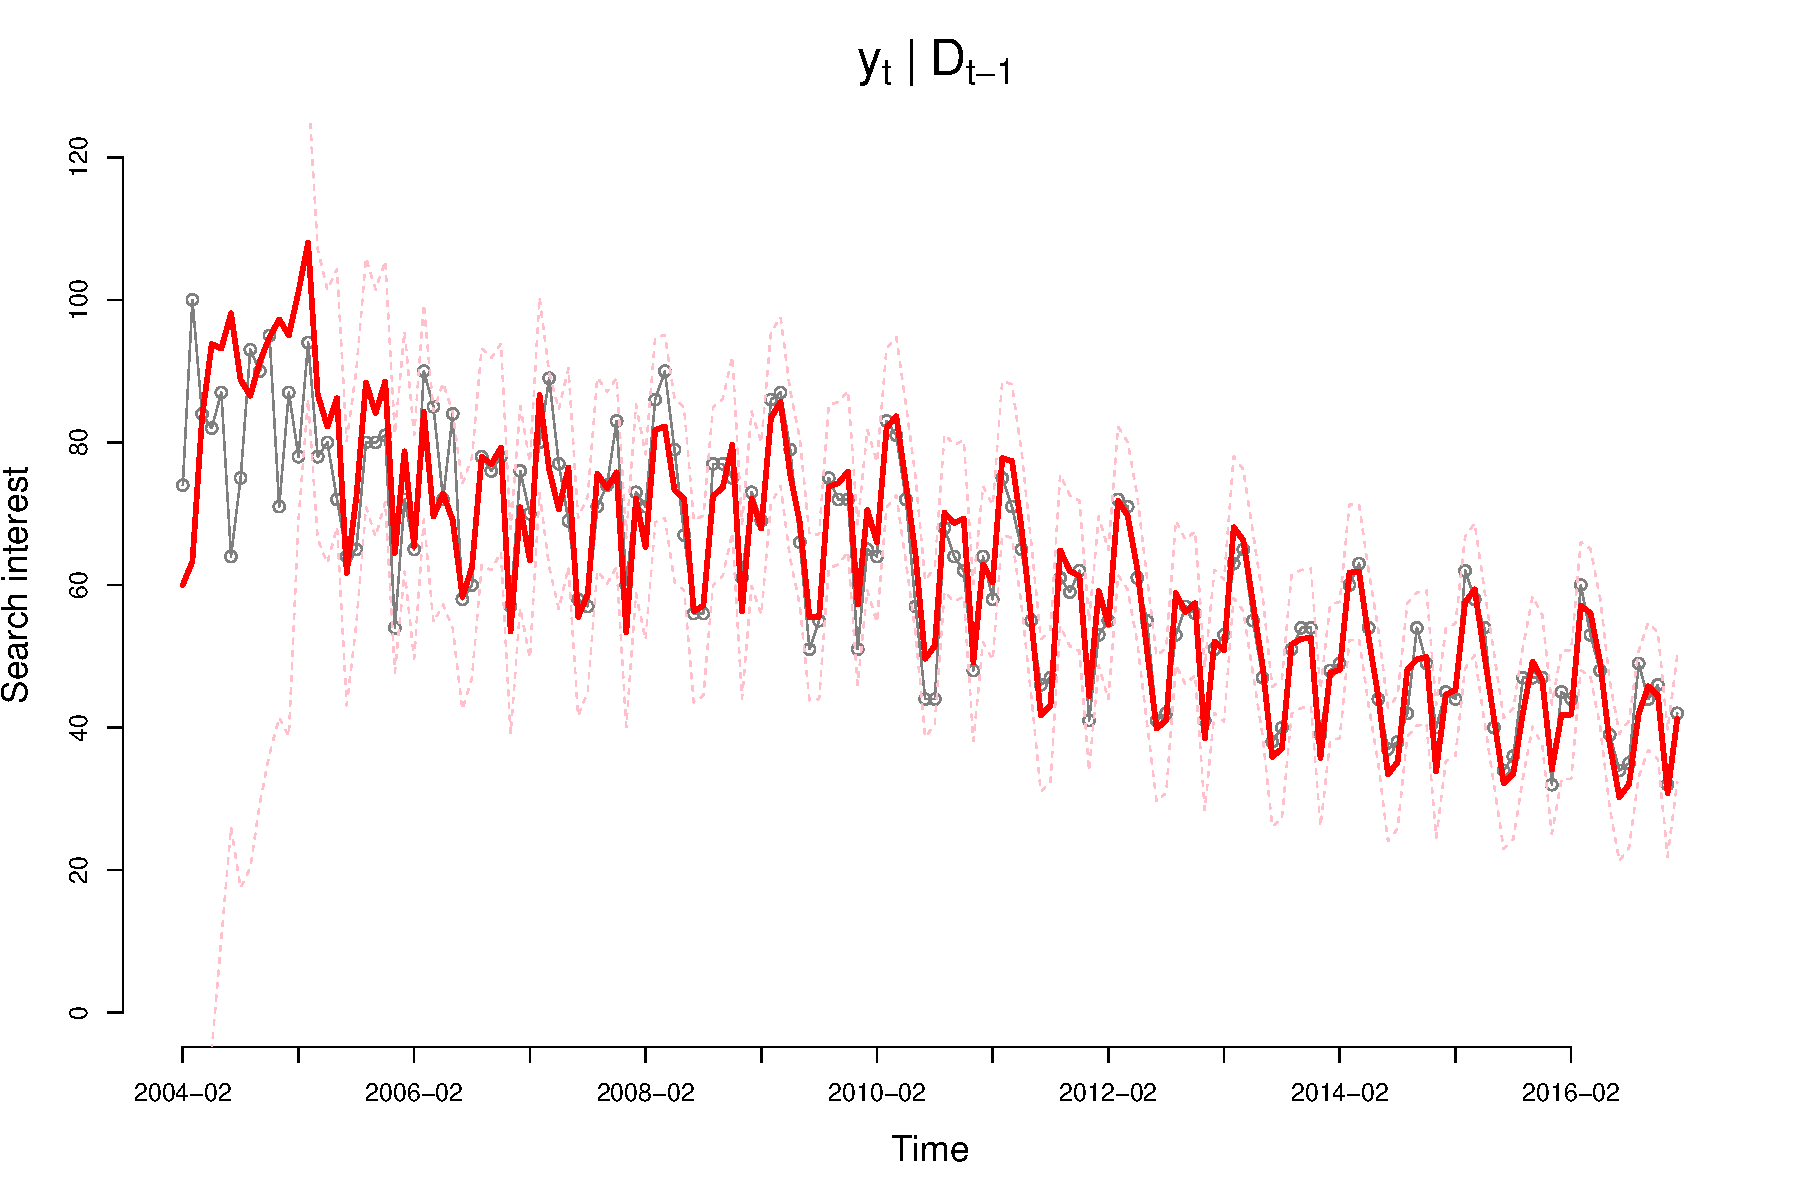
\includegraphics[scale=0.37]{figs/m1_onestep.pdf}
\end{center}
\caption{The gray dots mark the data. The thick red line is the mean forecast function and the thin dashed lines are 95\% credible intervals for $\mathcal{M}_1$.}
\end{figure}

\begin{figure}[H]
\begin{center}
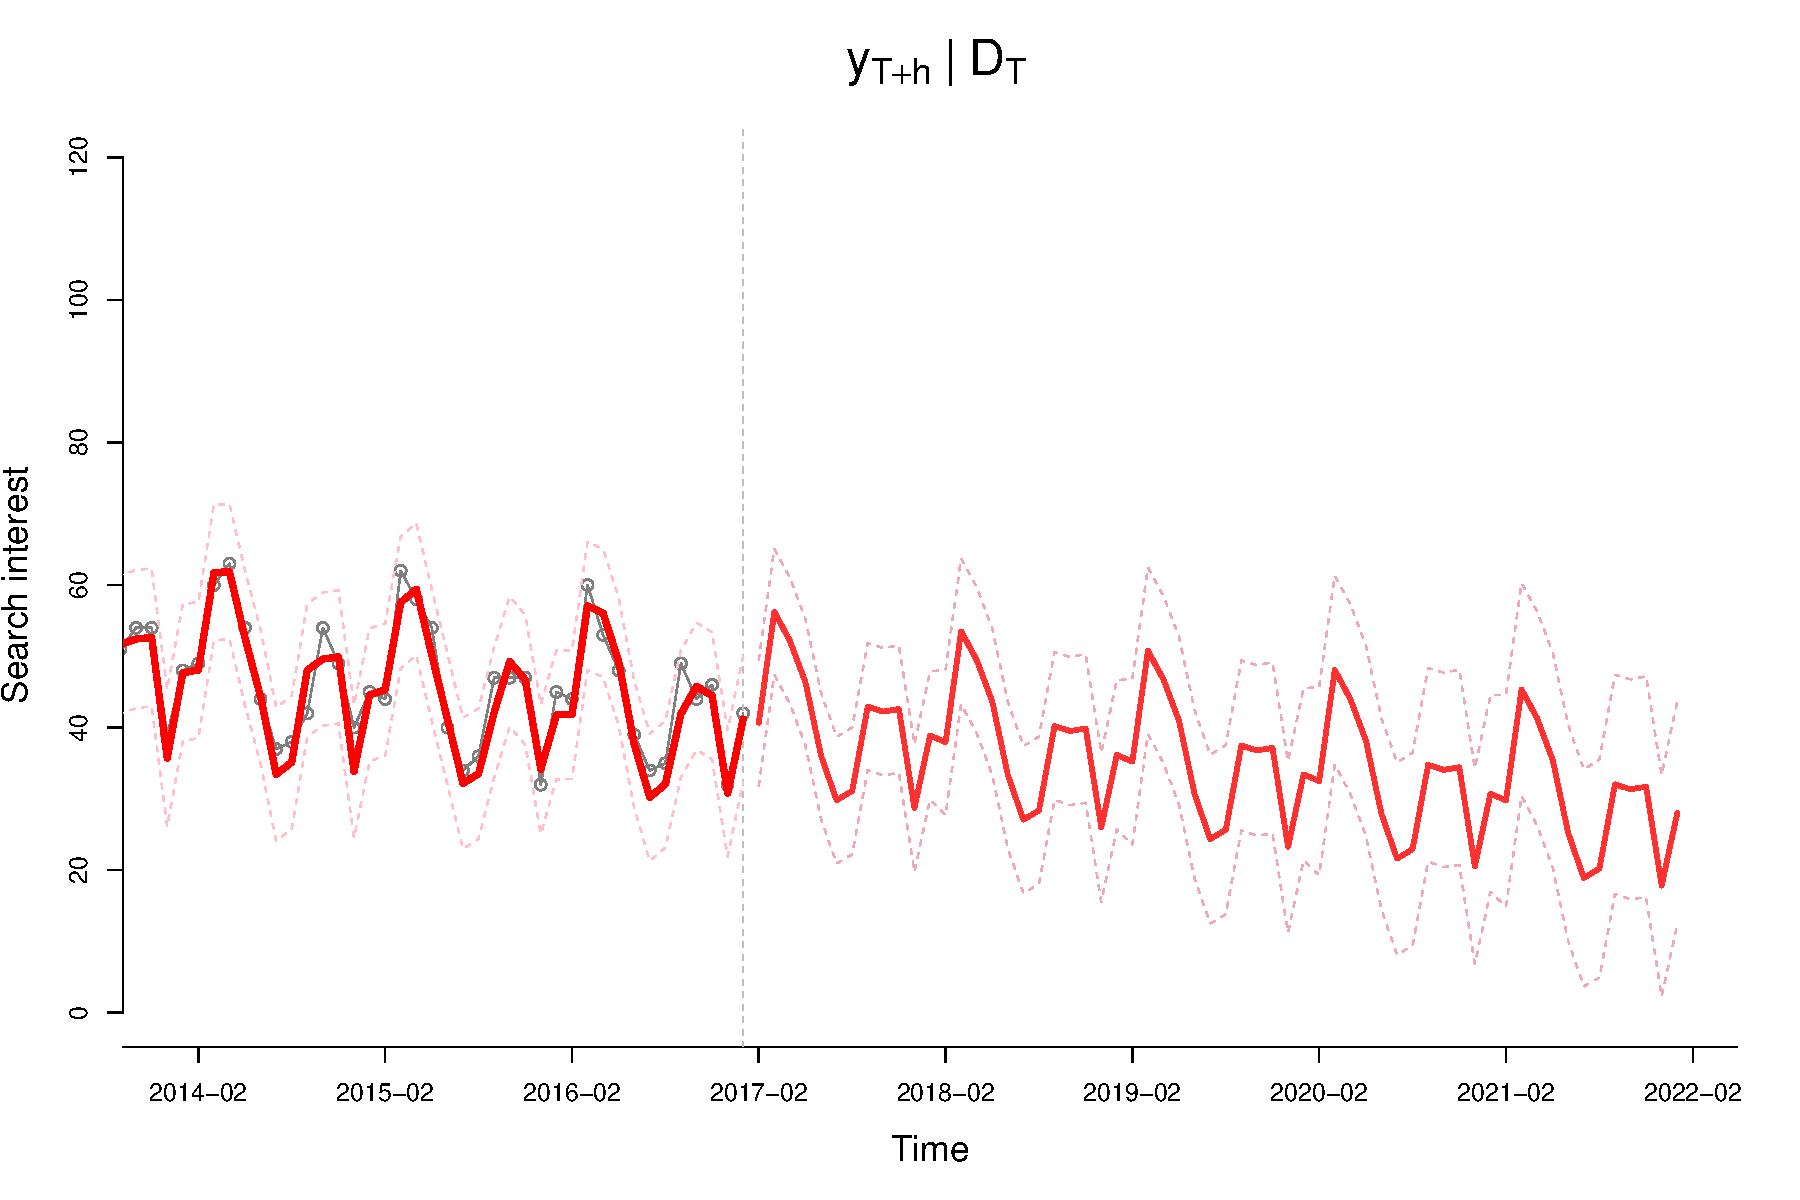
\includegraphics[scale=0.37]{figs/m1_forecast.pdf}
\end{center}
\caption{The five-year forecast for $\mathcal{M}_1$, for $h=1,\ldots,60$. The vertical line marks where the data end, picking up at the end of the plot in Figure 2.}
\end{figure}

\begin{figure}[H]
\begin{center}
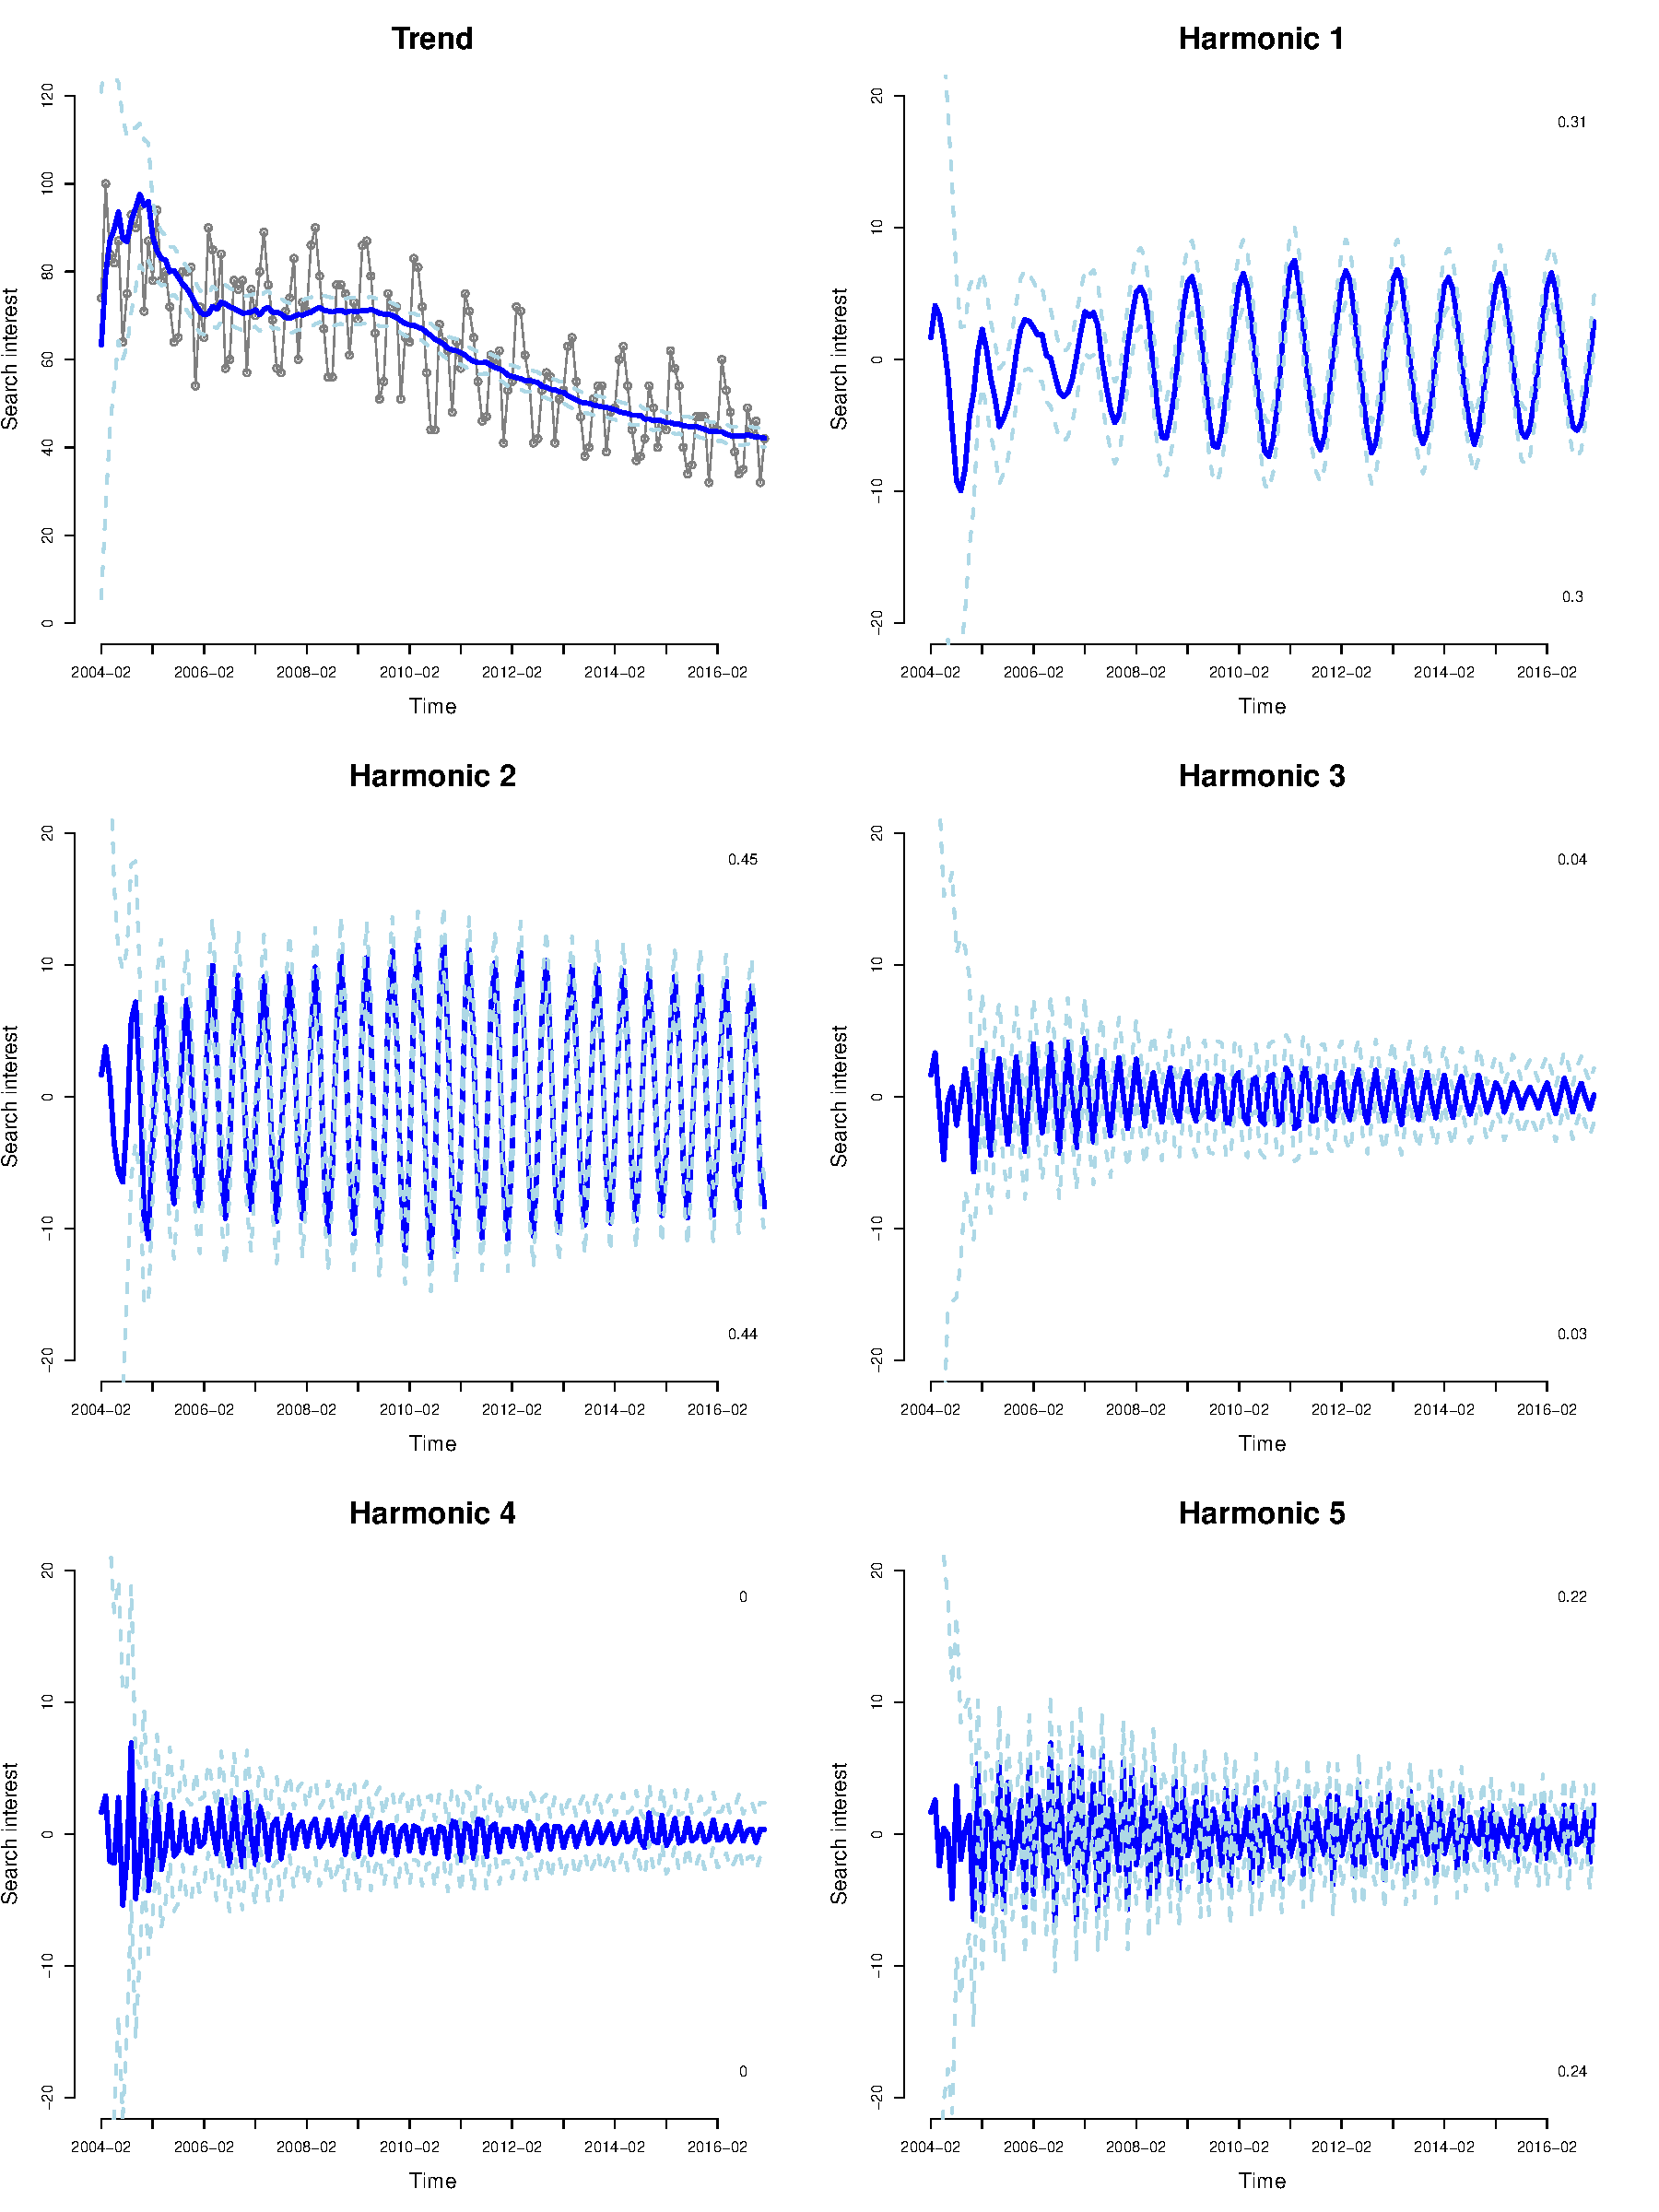
\includegraphics[scale=0.40]{figs/m1_components.pdf}
\end{center}
\caption{The trend and seasonal components for $\mathcal{M}_1$. The little numbers in the top right for the harmonic plots indicate the proportion of times the upper bound from the 95\% interval fell below zero. The little numbers in the bottom right are for the lower bound going above zero.}
\end{figure}

\begin{figure}[H]
\begin{center}
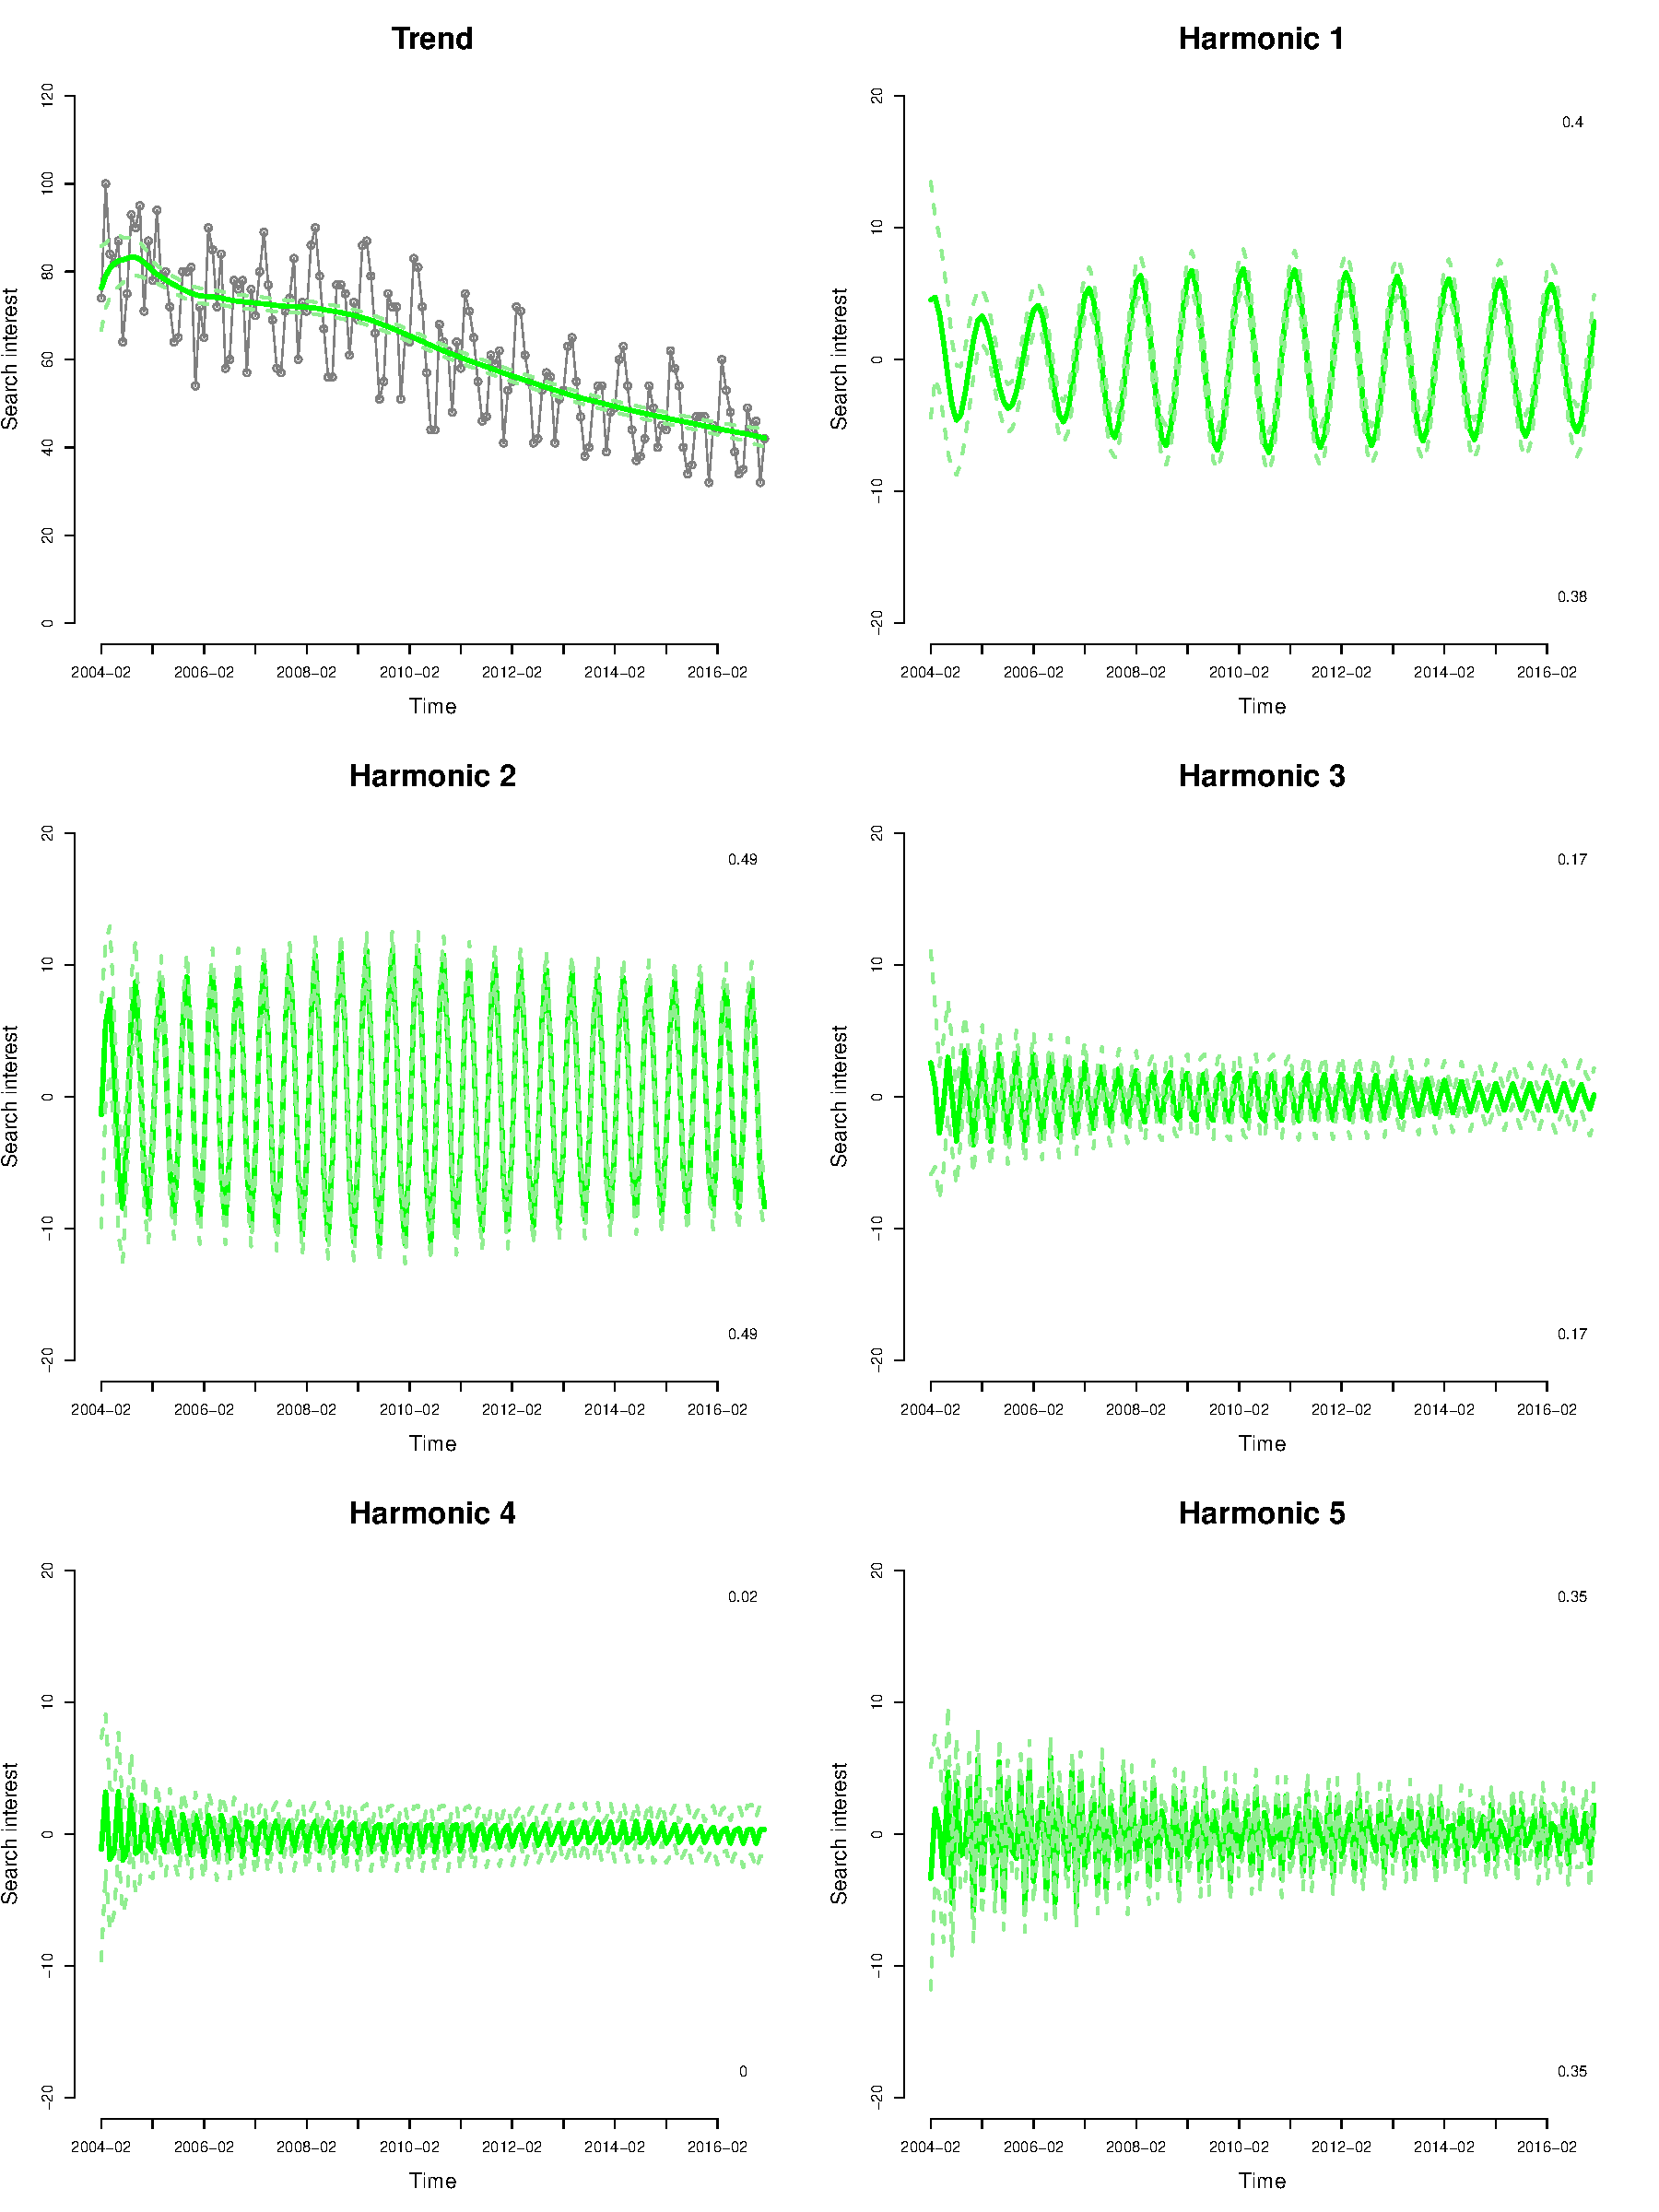
\includegraphics[scale=0.40]{figs/m1_smooth_components.pdf}
\end{center}
\caption{Same as in Figure 4, but for the smoothing distributions.}
\end{figure}

\newpage
\noindent The forecast distribution seems to be much more reasonable than what we saw from $\mathcal{M}_0$ which was constant for all $t>T$. The forecast in $\mathcal{M}_1$ continues the downward trend that we're seeing in the data as well as the cyclical behavior. A deficiency in our forecast function (and our model) is that we do not account for the bounds. If this forecast function were to have its way, we would see the search interest for UCSC fall to oblivion, being not worth more than a bare mention.
\bigskip

\noindent Consider the distribution of the harmonics given in Figure 5. We see that harmonics 1, 2, and 5, have 95\% intervals that cross zero at least 30\% of the time (marked by the little numbers on the right side of the plots). Harmonic 4 rarely cross zero, suggesting that it is unimportant since it may as well be a straight line. Harmonic 3 crosses zero about 17\% of the time, providing some evidence that this harmonic is unimportant. We discard harmonics 3 and 4 and perform the analysis.
\bigskip

\noindent The reduced model has a similar $\m{F}$ and $\m{G}$ except in $\m{F}$ the fourth and fifth $\m{E}_2^\top$ are omitted and $\m{G}_3$ and $\m{G}_4$ are omitted from $\m{G}$. We obtain a discount factor of $\hat{\delta}_2=0.952$ which evaluates to a log observed predictive density at $\log p_2(\m{y}|\mathcal{D}_0)=-482.3$, $3.4$ less than that of $\mathcal{M}_1$. The summary of distributions in Figure 6 through 9 are highly comparable to those from $\mathcal{M}_1$.
\bigskip

\noindent Since the removal of harmonics 3 and 4 result in only a small decrease in the log observed predictive density, we would say that the reduced model $\mathcal{M}_2$ is as useful as $\mathcal{M}_1$.

\newpage
\begin{figure}[H]
\begin{center}
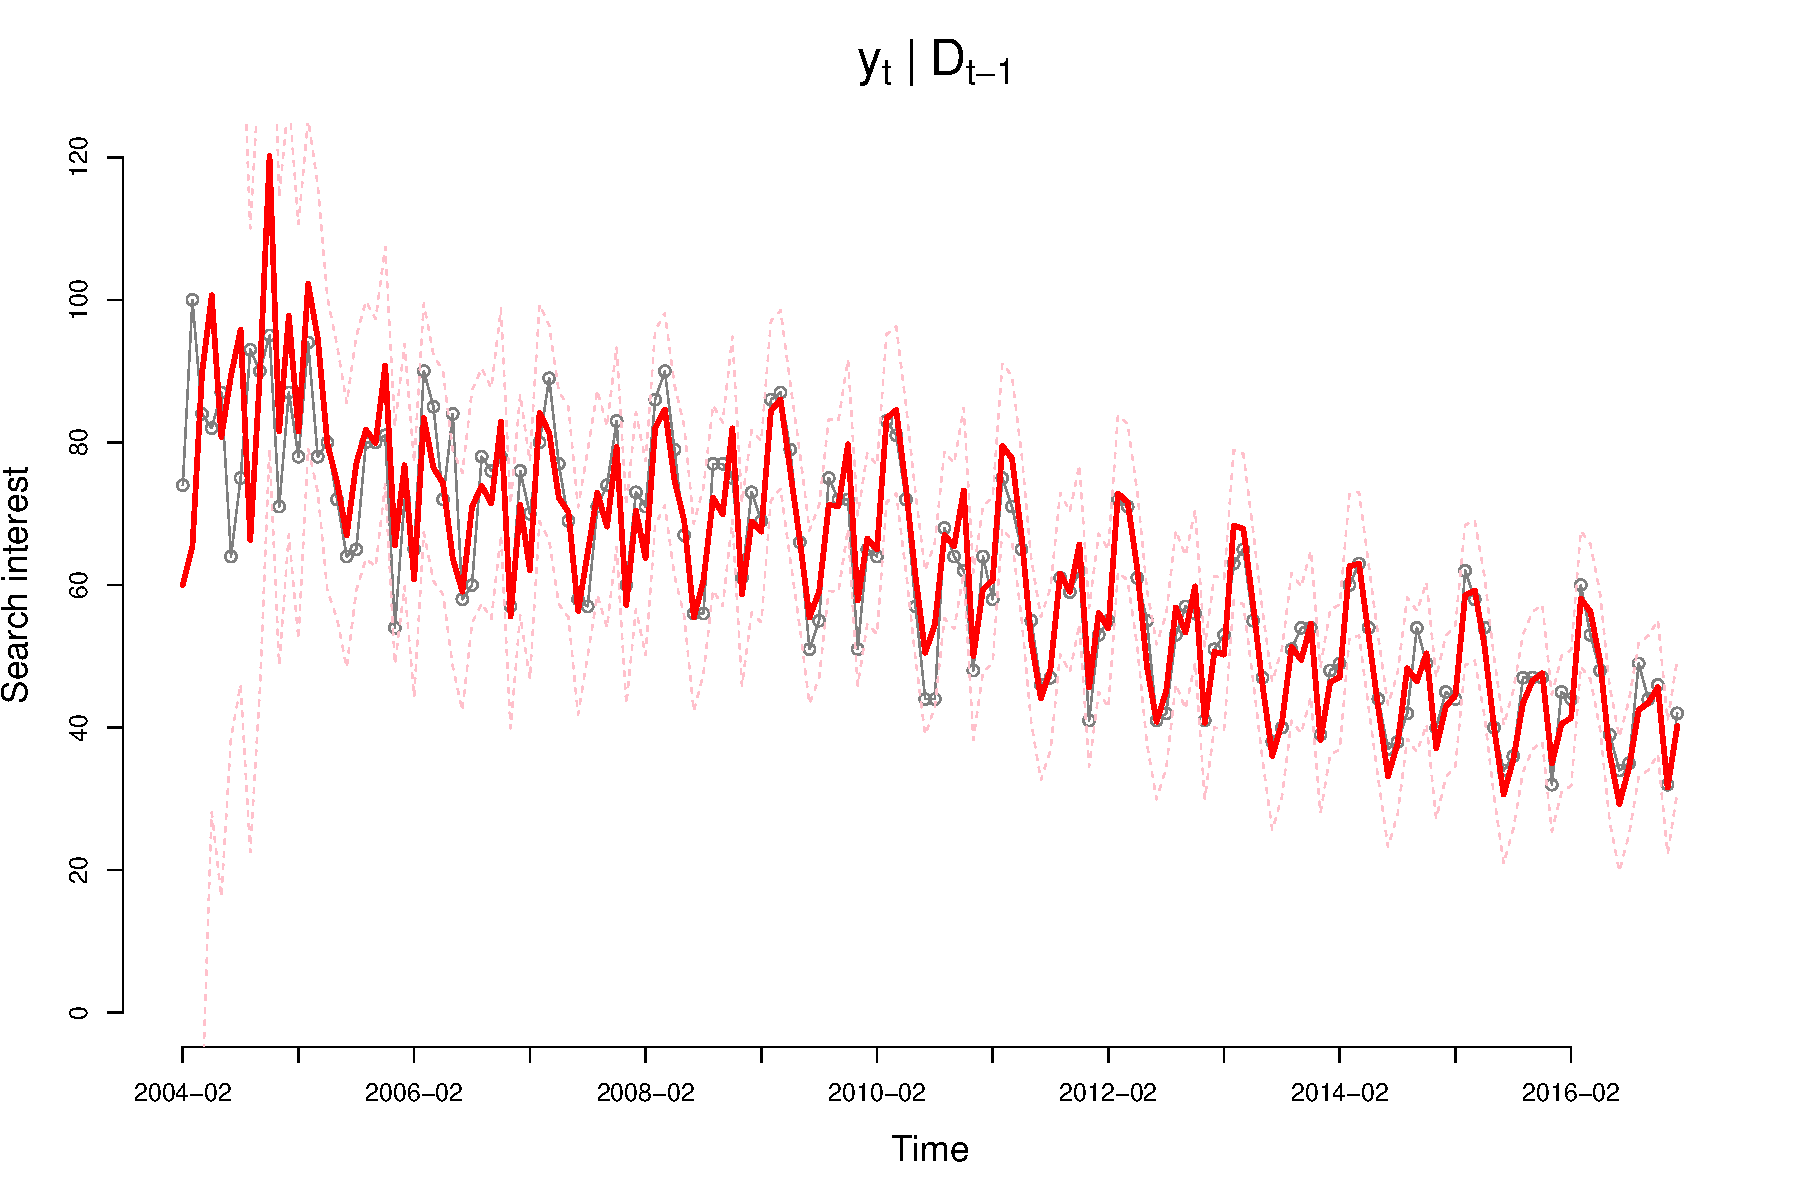
\includegraphics[scale=0.37]{figs/m2_onestep.pdf}
\end{center}
\caption{The gray dots mark the data. The thick red line is the mean forecast function and the thin dashed lines are 95\% credible intervals for $\mathcal{M}_2$.}
\end{figure}

\begin{figure}[H]
\begin{center}
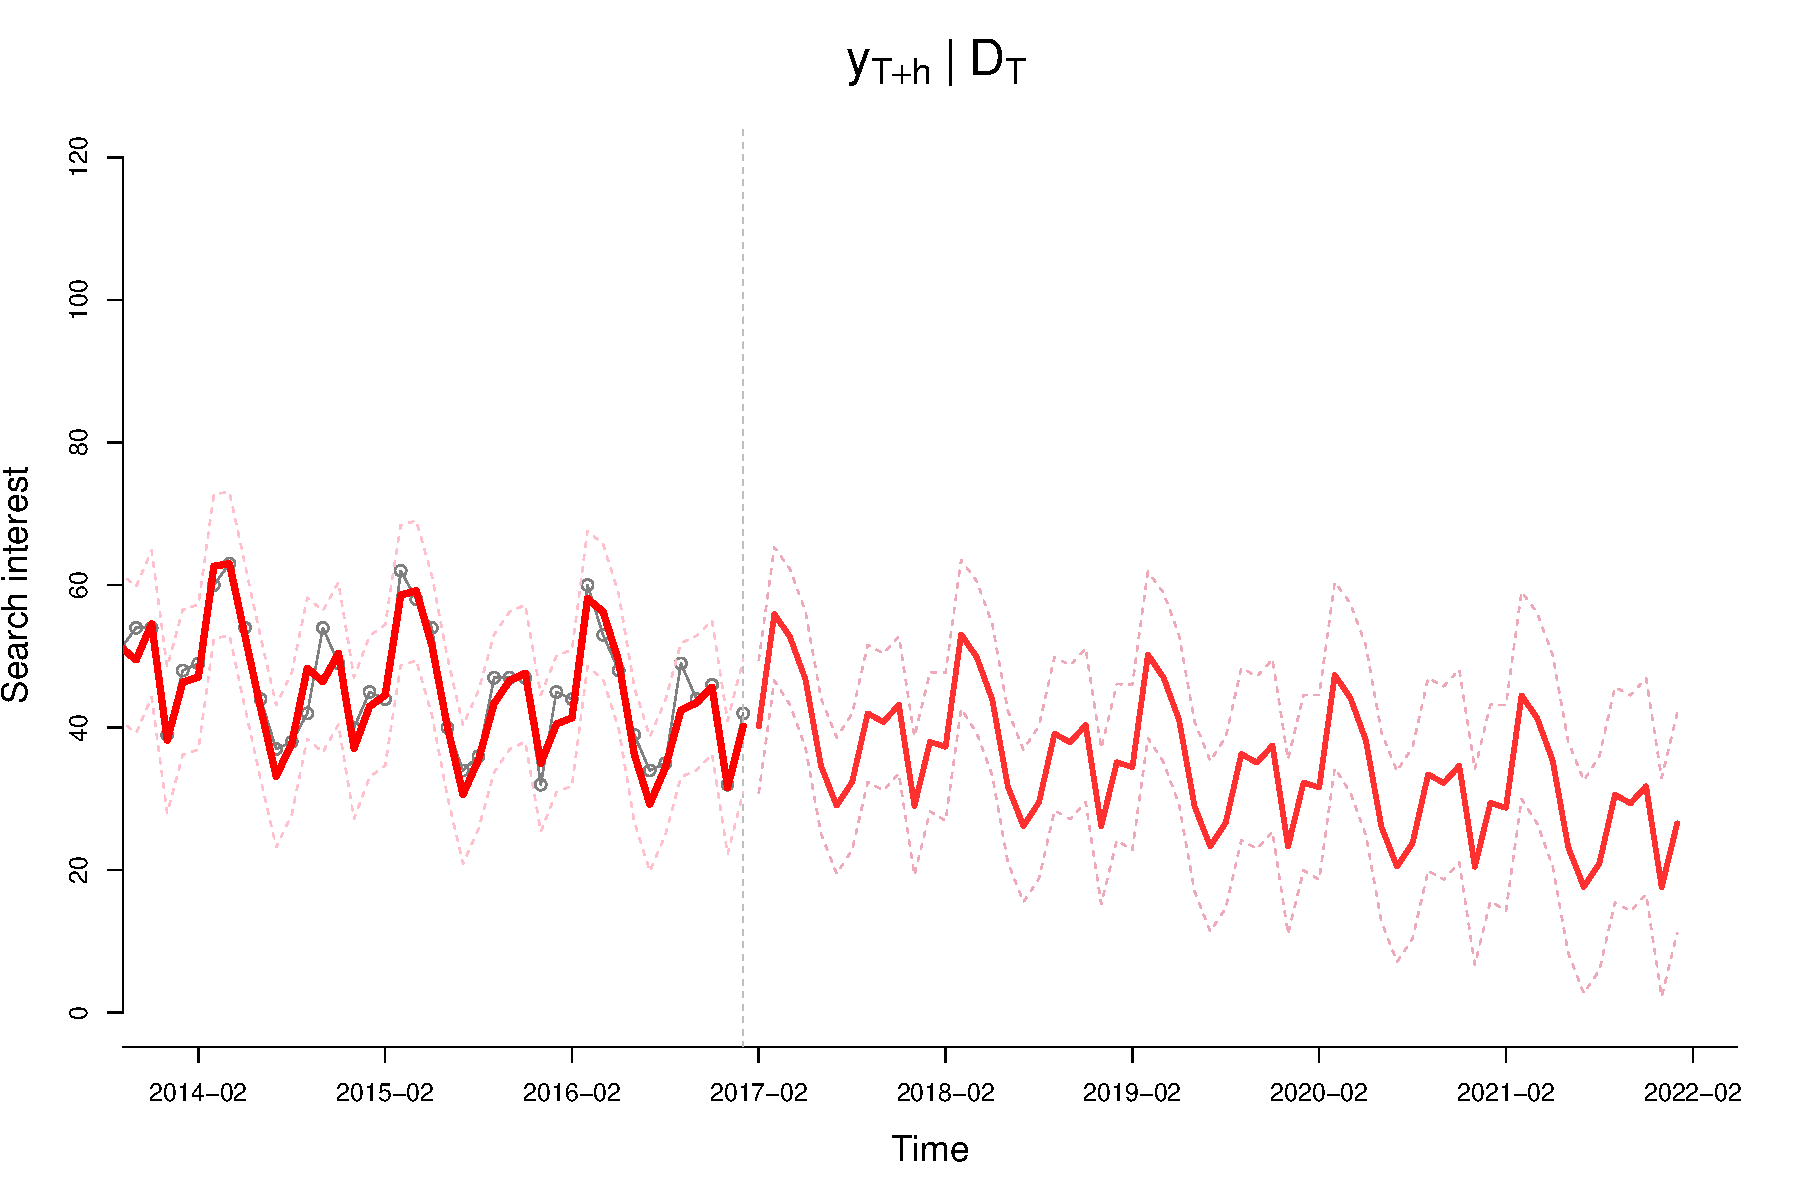
\includegraphics[scale=0.37]{figs/m2_forecast.pdf}
\end{center}
\caption{The five-year forecast for $\mathcal{M}_2$, for $h=1,\ldots,60$. The vertical line marks where the data end, picking up at the end of the plot in Figure 6.}
\end{figure}

\begin{figure}[H]
\begin{center}
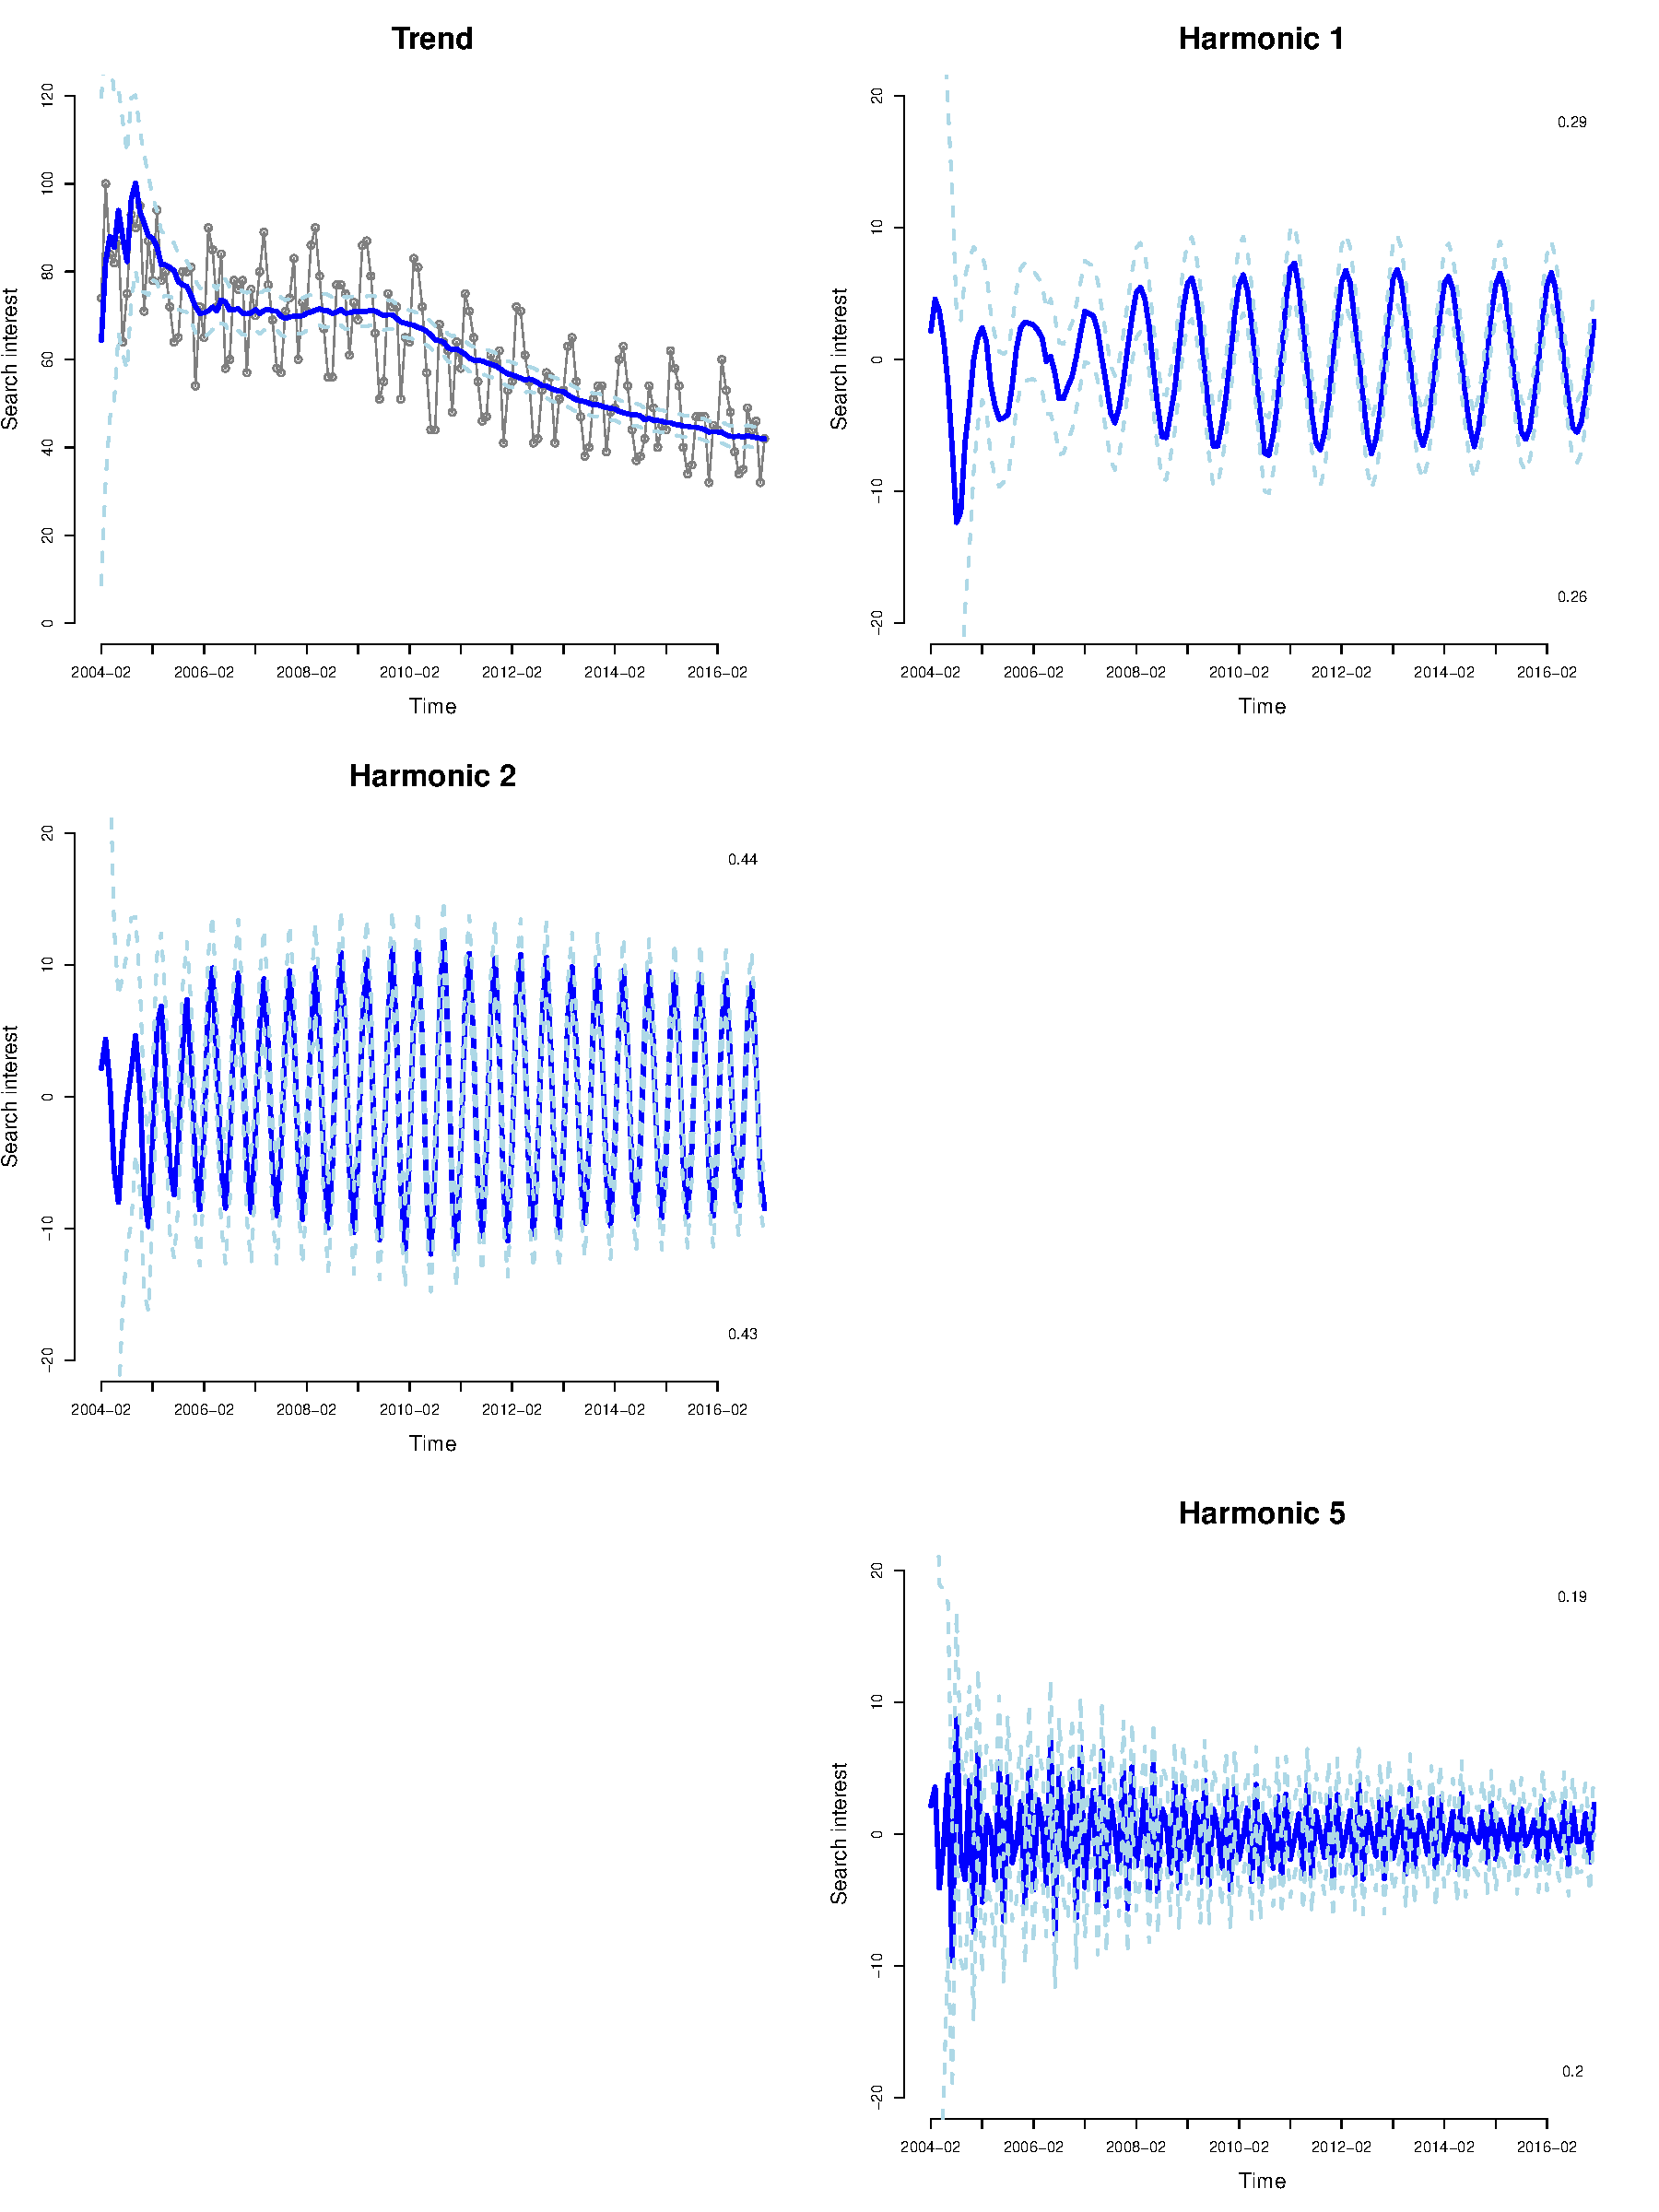
\includegraphics[scale=0.40]{figs/m2_components.pdf}
\end{center}
\caption{The trend and seasonal components for $\mathcal{M}_2$. The little numbers in the top right for the harmonic plots indicate the proportion of times the upper bound from the 95\% interval fell below zero. The little numbers in the bottom right are for the lower bound going above zero.}
\end{figure}

\begin{figure}[H]
\begin{center}
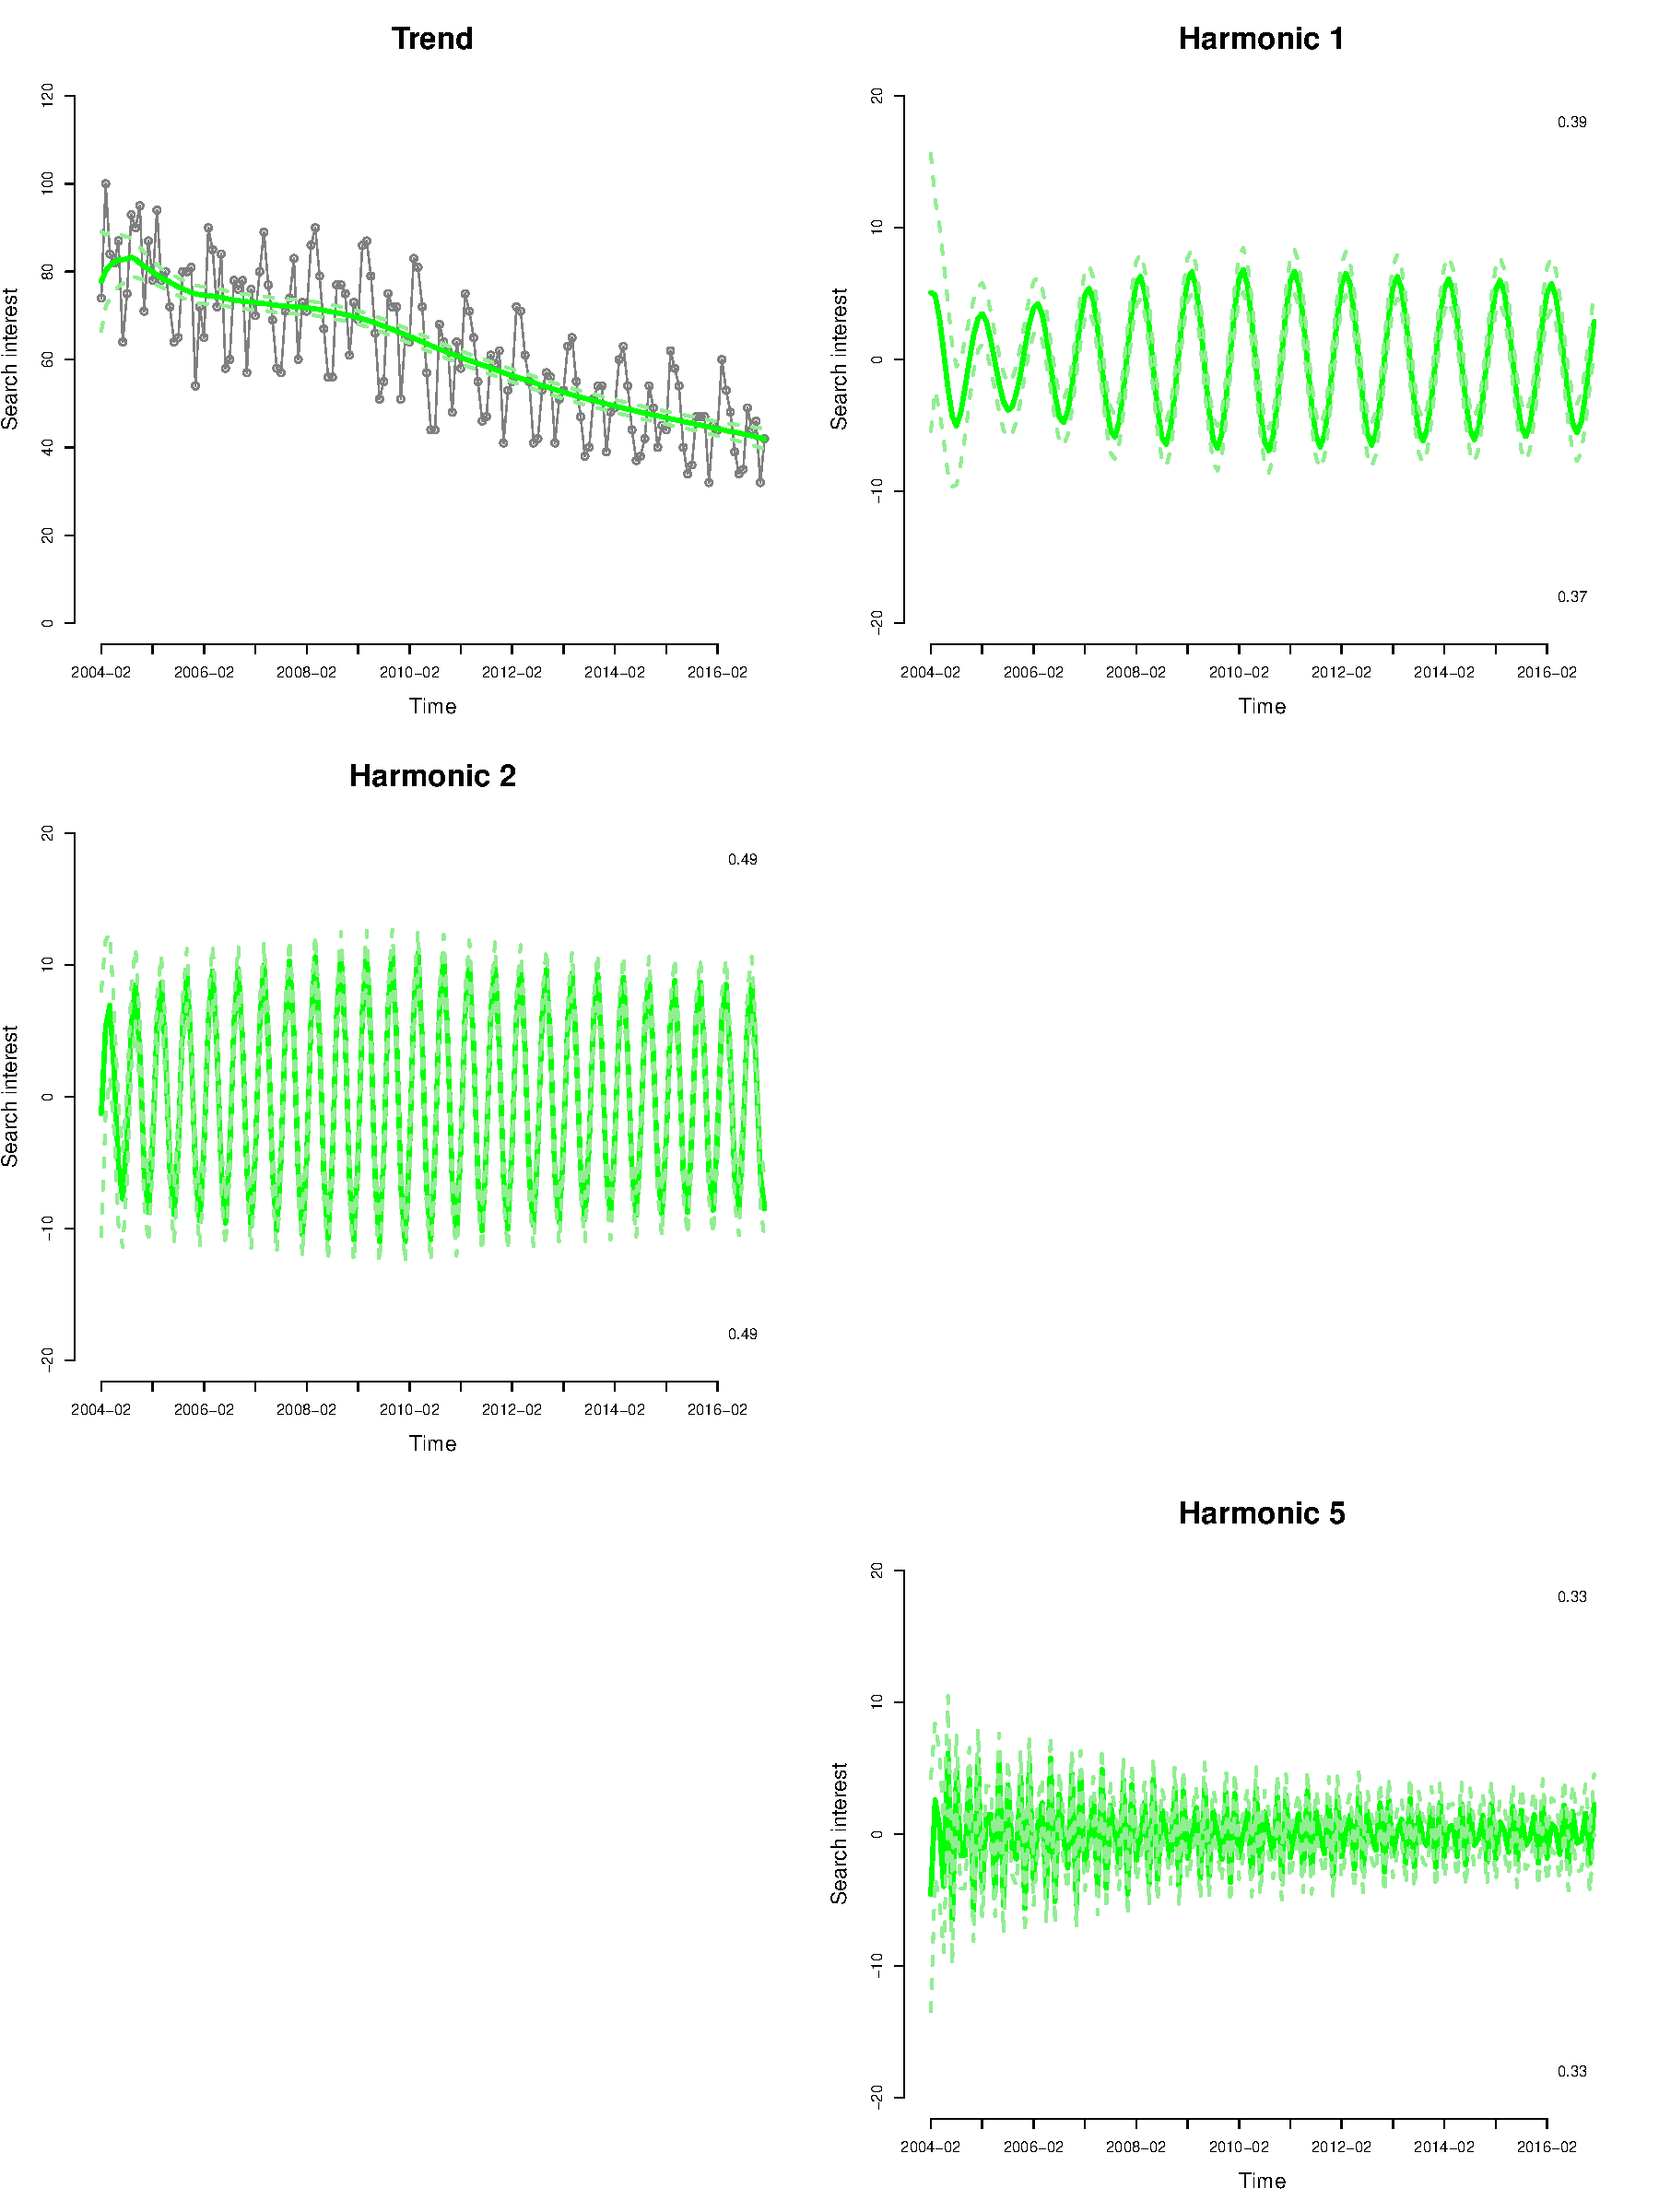
\includegraphics[scale=0.40]{figs/m2_smooth_components.pdf}
\end{center}
\caption{Same as in Figure 8, but for the smoothing distributions.}
\end{figure}

\newpage

\subsection*{Algorithm for fitting $\mathcal{M}_3$}

\noindent Model $\mathcal{M}_3$ is as follows:
\begin{align*}
y_t &= \alpha + \beta t + x_t + \epsilon_t,~~~~~\epsilon_t \sim N(0, v), \\
x_t &= \sum_{j=1}^q\phi_j x_{t-j} + \nu_t,~~~~~\nu_t \sim N(0, 30)
\end{align*}
\noindent with $\alpha \sim N(0, vw)$, $\beta\sim N(0, vw)$, and $v$, $w$ unknown and $q$ known.
\bigskip

\noindent The conjugate prior for $v$ is the inverse gamma, $v\sim IG(a_v, b_v)$, as well as for $w$, $w\sim IG(a_w, b_w)$. We let $x_{1-j}\sim N(m_j, C_j)$, for $j=1,\ldots,q$ be the priors for $x_0,x_{-1},\ldots,x_{1-q}$. Since $\m{\phi}$ are (conditional on $\m{x}$) AR coefficients, a good prior to use is $\m{\phi}\sim N(\m{m}_\phi, \m{C}_\phi)$, subject to being in the stationary region.
\bigskip

\noindent We obtain posterior samples for $(x_{1:T}, \alpha, \beta, \m{\phi}, v, w)$ with the following algorithm.
\begin{enumerate}
\item Initialize $(x_{1:T}^{(0)}, \m{\phi}^{(0)}, v^{(0)}, w^{(0)})$. Set $i=0$.
\item Increment $i$ by 1.
\item Sample $(\alpha^{(i)}, \beta^{(i)})^\top=\m{\mu}^{(i)}$ from

$\pi(\m{\mu}|\cdot) \propto N(\m{y}-\m{x}^{(i-1)}|\m{Z}_T\m{\mu}, v^{(i-1)}\m{I}_T)N(\m{0}, v^{(i-1)}w^{(i-1)}\m{I}_2)$, where the rows of $\m{Z}_T$ are $(1, t)$, for $t=1,\ldots,T$.
\item Sample $v^{(i)}$ from $v|\cdot \sim IG\left(a_v, b_v + \frac{1}{2}(K + (\alpha^{(i)})^2/w^{(i-1)} + (\beta^{(i)})^2/w^{(i-1)})\right)$ where $K=(\m{y}-\m{x}^{(i-1)}-\m{Z}_T\m{\mu}^{(i)})^\top(\m{y}-\m{x}^{(i-1)}-\m{Z}_T\m{\mu}^{(i)})$.
\item Sample $w^{(i)}$ from $w|\cdot \sim IG\left(a_w, b_w + \frac{1}{2}((\alpha^{(i)})^2/v^{(i)} + (\beta^{(i)})^2/v^{(i)})\right)$.
\item Since, conditional on $\m{\phi}^{(i-1)}$, we have a DLM, then we sample from $\m{x}^{(i)}$ using FFBS. Use the recursion formulas to get $\pi(x_t|\mathcal{D}_t,\cdot)$, then obtain the smoothing distributions $\pi(x_t|\mathcal{D}_T,\cdot)$, for $t=T:1$. Sample $x_t^{(i)}$ from $\pi(x_t|\mathcal{D}_T,\cdot)$, where $(\cdot)$ denotes the most recent samples from the other parameters.
\item Sample $\m{\phi}^{(i)}$ using a Metropolis-Hastings step. The function used in the M-H ratio is $\pi(\m{\phi}|\m{x},\cdot)\propto \pi(\m{\phi})\prod_{t=1}^T N(x_t|\sum_{i=1}^j\phi_j x_{t-j}, 30)$
\item Go to step 2 until $i=B$, for some large $B$.
\end{itemize}

\end{document}
